\newpage
\section*{Earls of Ravnica}

\subsection*{The \texttt{district} module}

I have chosen to use the \texttt{gen\_statem} behaviour for my implementation. An individual district is its own state machine, and so, it makes sense to model it as such using the \texttt{gen\_statem} behaviour in Erlang. The callback mode i have used is \texttt{state\_functions}. That is, for each state of the district I define a callback function to handle the variaous events. This is, in my opinion, more convenient than using \texttt{handle\_event\_function}, since you can have a dedicated function per state.

I will try to cover only the most essential parts of my implementation, leaving the rest as something to read in the source.

\paragraph{Creating a district} In order to create a district, and thus initialize a new state machine, I have implemented \texttt{create} by simply calling \texttt{gen\_statem:start}, giving the module name, description, and the empty list as arguments. The \texttt{init} callback function sets the inital state to \texttt{under\_configuration} and passes the initial state data. Since we are working with neighbours, creatures, a trigger, and a description as the state data, the data is represented by a four-tuple consisting of a \texttt{map(atom() => passage())}  for the neighbours, a \texttt{map(creature\_ref() => creature\_stats())} for the creatures, simply a \texttt{trigger()} function for the trigger, and a string for the description. Maps make it easy to maintain a collection of pairs where each key is unique, and the lookup is easy and efficient.

% \paragraph{Getting the description} This simply sends a call to the given district, which will then return the description from the state data no matter the state in which it is.

\paragraph{Connecting districts} \texttt{connect} sends a call to the given district, passing the action and the destination. Representing the connections to the neighbours as a map, it is easy see if the action is already taken; simply ask if the action already exists as a key, and if it does, return the appropriate error. Else, put it into the map with the destination as the value and return \texttt{ok}.

\paragraph{Activating a district} This has been a bit tricky, and I have tried a few solutions before choosing to do it this way. When a district, which is under configuration, is activated, it immediately goes to the \texttt{under\_activation} state and forces the next event to be an internal event where the district then activates all of its neighbours. When each activation of the neighbours has returned a value, the district checks if any activation has been impossible. If this is the case, the district itself can't be activated. In order to avoid blocking the processes, each path that is activated keeps track of a list of visited districts. Thus, everytime a district is activating its neighbours, it chooses to ignore the ones that have already been visited. This also takes care of cycles, however, even without the list of visited districts, cycles are handled automatically; \texttt{activate} terminates the chain of calls when it is already under activation.

If there is a path from the root district being activated to some district that can't be activated, the root district also fails. Thus, I assume that it is possible to activate a part of a territory that does not include the root being activated. On Figure \ref{fig:activate} I have tried to illustrate my assumption about how \texttt{activate} would work. A, B, and (trivially) C fail to activate since they all have a path to a district that can't be activated. However, D and E are successfully activated.
\begin{figure}
  \centering
  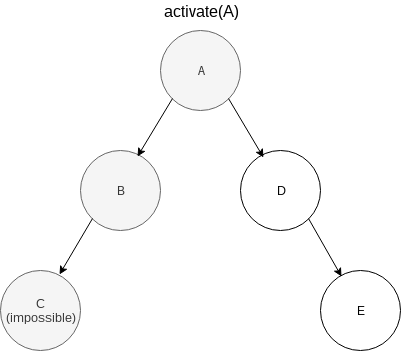
\includegraphics[width=0.5\textwidth]{figures/activate}
  \caption{Activating a district A with one path to a district that can't be activated and one path without problems.}\label{fig:activate}
\end{figure}

\paragraph{Entering a district} This sends a call to the district, passing the creature wanting to enter. The district simply checks to see if the reference is already a key in the creature map, and if not, applies the \texttt{entering}-trigger to the creature entering and the creatures already in the district. The result then represents the  new map of creatures in the state data.

The way the well-formedness of the trigger is checked is as follows. A new process applying the trigger is spawned, which sends a message back with the result. This allows me to use the \texttt{after}-timeout when receiving the result. If there is no result within 2 seconds, the input to the trigger is simply returned. The spawned process calls the trigger and catches any exception that may occur --- if this happens, the input is returned. If there is a response within 2 seconds, the check proceeds by ensuring that the result is a tuple, and that all the creature references are the same. If all is well, the new data is returned. There is no check on the use of functions inside the trigger, so it is possible for trigger to call an API function. This may cause problems if a district applies a trigger that makes a call to this very district, perhaps blocking the process.

\paragraph{Taking action} This sends a call to the district, passing the creature reference and the action. The district makes sure that the creature is actually in the map of contained creatures and that the action exists in the map over neighbours. If so, the \texttt{leaving}-trigger is applied to the creature leaving and the creatures staying in the district, and \texttt{enter} is called on the destination. If all goes well, the creature is moved. One special case is when the action is an edge to the same district; this would, again, block everything. Thus, if the destination is the same as the current district, the \texttt{entering}-trigger is applied locally and the state data is updated accordingly.

This solution may not be the most elegant since it repeats some code from \texttt{enter}. However, given the problems that arise when handling self loops, this solution is a very simple way to avoid blocking the process.

\paragraph{Shutting down a district} This works much in the same way as \texttt{activate}. After sending the required message to the \texttt{NextPlane} argument, the district immediately goes to the \texttt{shutting\_down} state and forces an internal event that makes it shut down its neighbours. After they have all been visited, It uses the \texttt{gen\_statem:stop} to actually terminate the process.




\subsection*{Testing \texttt{district}}

I have already gone over some reasons why my implementation should behave correctly. To further ensure the behavour of my implementation, I have written some unit tests and some property-based tests.

\paragraph{Unit testing} I have chosen to do a series of unit tests much like I did in Haskell. In case the property-based QuickCheck tests are not producing good enough instances, at least these unit tests can tell a bit about the integrity of each part of the implementation. I chose to use EUnit for this task, since it is simple and easy to use, and its error messages when tests fail are very helpful.

There are 50 unit tests which, collectively, cover all requirements from the assignment. These range from connecting districts, moving a creature from a district to another, activating territories with cycles and self loops, registering well-formed triggers and triggers returning ill-formed data and throwing exceptions, and shutting down while checking the messages afterwards. In my opinion, these tests show that the behaviour of my implementation is at least pretty close to the intended behaviour described in the assignment. The fact that all tests pass indicates that a large portion of the solution is correct. The tests can be found in \texttt{ravnica/district\_bb}.


\paragraph{QuickChecking the properties} I have written a territory generator that simply creates a random map as described in the assignment. I have also, as was the task, implemented \texttt{setup\_territory}, which takes this map and creates a district for each of the keys, creates all connections from the \texttt{\{atom(),key()\}} list, and finally returns all district pids as the resulting territory. I won't go into detail about the concrete implementations of these. An example of a generated territory (on the form before setting up the actual districts) can be seen in Appendix \ref{app:genter}. \\

\noindent In order to check the neighbours of and the creatures in the districts after calling som API function, I initially used \texttt{sys:get\_state}. However, I realized that this is heavily implementation-specific (how is the state data represented?), so I had to choose a much simpler, and not as flexible, approach.
Thus, I have implemented property-based for three API functions:
\begin{itemize}
  \item \texttt{activate}
  \item \texttt{shutdown}
  \item \texttt{take\_action}
\end{itemize}
When testing activation, I simply make sure that if we can successully activate some district in the generated territory, then the neighbours will be active afterwards. This is done by creating a creature and moving it to the neighbours. This gives me the pid of the neighbour, and I check the state using \texttt{sys:get\_state} (not relying on the state data, only the state itself). I could assume that moving the creature would be enough since it is only allowed when both the current district and the neighbour are active, but actually fetching the state is in my opinion a better indicator.

When testing the territory when shutting down, I activate some district in the generated territory, create a creature, move it to some neighbour, get the pid of said neighbour, shut down the current district, and check that both processes have terminated using \texttt{process\_info}. This would indicate that a district is actually correctly shut down.

When testing actions, I simply create a creature, enter it in some district from the generated territory, move it to a neighbour through an action, and then try to move it from the same district to a neighbour through the same action. This should fail, since the creature is no longer in the inital district.

\paragraph{Assessment} I realize that my specific property-based tests are not a sure guarantee that my implementation is perfect; they are rather simple, only testing within a very local neighbourhood in any generated territory. However, they still do show some qualities about my implementation that are required in a correct solution, so they are in my opinion far from worthless.

The unit tests, on the other hand, strongly indicate correct behaviour on various instances with intentional edge cases and errors. Here, not a single instance behaves unexpectedly as long as it is well-formed as per the assignment.
